% Chapter Chapter 4 For Reproducible Research in R and RStudio
% Christopher Gandrud
% Created: 16/07/2012 05:45:03 pm CEST
% Updated: 26 December 2012




\chapter{Getting Started with File Management}\label{DirectoriesChapter}

Careful file management is crucial for reproducible research. Remember two of the guidelines from Chapter \ref{GettingStartedRR}:

\begin{itemize}
    \item Explicitly tie your files together,
    \item Have a plan to organize, store and make your files available. 
\end{itemize}

\noindent Apart from the times when you have an email exchange (or even meet in person) with someone interested in reproducing your research, the main information independent researchers have about the procedures you used will be stored across many files: data files, analysis files, and presentation files. If these files are well organized and the links tying them together are clear, replication will be much easier. File management is also important for you as a researcher, because if your files are well organized you will be able to more easily make changes, benefit from work you have already done and collaborate with others. 

Using tools such as R, {\emph{knitr}}, and markup languages like LaTeX requires fairly detailed knowledge of where files are stored in your computer. Handling files reproducibly may require you to use command line tools to access and organize your files. R and Unix-like shell programs\index{Unix-like shell program} allow you to control files--creating, deleting, relocating--in powerful and really reproducible ways. By typing these commands you are documenting every step you took. This is a major advantage over graphical user interface-type systems where you organize files by clicking and dragging them with the cursor. However, text commands require you to know your files' specific addresses--their file paths. 

In this chapter we discuss how a reproducible research project may be organized and cover the basics of file path naming conventions\index{file path naming conventions} in Unix, Mac, and Windows systems. We then learn how to organize them with RStudio Projects\index{RStudio Projects}. Finally, we will cover some basic R and Unix-like shell commands for manipulating files as well as how to navigate through files in RStudio in the {\bf{Files}} pane. The skills you will learn in this chapter will be heavily used in the next chapter (Chapter \ref{Storing}) and throughout the book.

In this chapter we work with locally stored files\index{locally stored}, i.e. files stored on your computer. In the next chapter we will discuss various ways to store and access files remotely stored in the cloud\index{cloud storage}.


\section{File paths \& naming conventions}

All of the operating systems\index{operating systems} covered in this book organize files in hierarchical directories\index{directories}, also know as file trees. To a large extent, directories can be thought of as the folders you usually see on your Windows or Mac desktop.\footnote{To simplify things, I use the terms `directory' and `folder' interchangeably in this book.} They are called `hierarchical' because directories are located inside of other directories, as in Figure \ref{ExampleTree}. 

\subsection{Root directories}

A root directory\index{root directory} is the first level in a disk, such as a hard drive. It is the root out of which the file tree `grows'. All other directories are subdirectories\index{subdirectory} of the root directory.

On Windows computers you can have multiple root directories, one for each storage device or partition of a storage device. The root directory is given a drive letter assignment\index{drive letter assignment}. If you use Windows regularly you will most likely be familiar with the \texttt{C:\textbackslash{}} used to denote the C partition of the the hardrive. This is a root directory. On Unix-like systems, including Macs, the root directory is simply denoted by a forward slash (\texttt{/}) with nothing before it.

\subsection{Subdirectories \& parent directories}

You will probably not store all of your files in the root directory. This would get very messy. Instead you will likely store your files in subdirectories of the root directory. Inside of these subdirectories may be further subdirectories and so on.  Directories inside of other directories are child directories\index{child directories} or subdirectories of a parent directory\index{parent directory}.

On Windows computers separate subdirectories are indicated with a back slash (\textbackslash{}). For example if we have a folder called {\emph{Data}} inside of a folder called {\emph{ExampleProject}} which is located in the C root directory it has the address \texttt{C:\textbackslash{}ExampleProject\textbackslash{}Data}.\footnote{For more information on Windows file path names see this helpful website: \url{http://msdn.microsoft.com/en-us/library/windows/desktop/aa365247(v=vs.85).aspx}} When you type Windows file paths into R you need to use two backslashes rather than one: \texttt{C:\textbackslash{}\textbackslash{}ExampleProject\textbackslash{}\textbackslash{}Data}. This is because the \texttt{\textbackslash{}} is an escape character\index{escape character} in R.\footnote{As we will see in Part IV, it is also a LaTeX escape character.} Escape characters tell R to interpret the next character or sequence of characters differently. For example, on page \pageref{TSVEscape} you'll see how \texttt{\textbackslash{}t} can be interpreted by R as a tab rather than the letter ``t''. Add another escape character to neutralize the escape character so that R interprets it as a backslash. In other words use an escape character to the escape character. Another option for writing Windows file names in R is to use one forward slash (\texttt{/}).  

On Unix-like systems, including Mac computers, directories are indicated with a forward slash (\texttt{/}). The file path of the {\emph{Data}} file on a Unix-like system would be: \texttt{/ExampleProject/Data}

In the book I switch between the two file system naming conventions to expose you to both.

\subsection{Spaces in directory \& file names}

It is generally good practice to avoid putting spaces in your file and directory names. For example, I called the example project parent directory ``ExampleProject" rather than ``Example Project". Spaces in file and directory names can sometimes create problems for compter programs trying to read the file path. It may believe that the space indicates that the path name has ended. To make multi-word names easily readable without using spaces, adopt a convention such as CamelBack\index{CamelBack}. In CamelBack new words are indicated with capital letters, while all other letters are lower case. For example, ``ExampleProject".

\subsection{Working directories}

When you use R and markup languages it is important to keep in mind what your current working directory is\index{working directory}. The working directory is the directory where the program automatically looks for files and other directories, unless you tell it to look elsewhere. It is also where it will save files. Later in this chapter we will cover commands for finding and changing the working directory.

\section{Organizing your research project}

Figure \ref{ExampleTree} gives an example of how the files in a simple reproducible research project could be organized. The project's main parent directory is called {\emph{ExampleProject}}. Inside this directory are three subdirectories: a data gathering directory, an analysis directory, and a presentation directory. Each of these directories contains further subdirectories and files. The {\emph{Presentation}} directory for example contains subdirectories for files that present the findings in article, slideshow, and website formats.

\clearpage
\thispagestyle{plain}
\begin{landscape}
\begin{figure}[th!]
    \caption{Example Research Project File Tree}
    \label{ExampleTree}
    \begin{center}
    
    \documentclass{article}

\usepackage{tikz}

\begin{document}

%%%%%% Example 

\tikzstyle{DirBox} = [draw=black, rectangle, minimum width=5em, thick]
  
\begin{tikzpicture}
  % Root Directory
  \node (root) at (5, 10) [DirBox]{Root};
  
  % Project Directory
  \node (project) at (5, 8.5) [DirBox]{Project};
  
  % Main Project sub-directories
  \node (data) at (2, 7) [DirBox]{Data};
  \node (analysis) at (5, 7) [DirBox]{Analysis};
  \node (presentation) at (8, 7) [DirBox]{Presentation};
  
  % Data subdirectories/files
  \node (dataGatherSource) at (-0.5, 6) [DirBox]{GatherSource};  
  \node (dataFiles) at (2, 6) [DirBox]{DataFiles};
  
  \node (dataMake) at (-0.5, 5.25) {{\small{DataMakeFile.R}}};
  
  \node(dataGather) at (-0.5, 4.5) [DirBox]{IndvDataGather};
  \node (dataGather1) at (-0.5, 3.5) {{\small{DataGather1.R}}};
  
  % Analysis subdirectores/files
  
  % Presentation subdirectories/files
  
  % Connect boxes
  \draw (root) -- (project);
  \draw (project) -| (data);
  \draw (project) -- (analysis);
  \draw (project) -| (presentation);
  
  %% Data connect boxes
  \draw (data) -| (dataGatherSource);
  \draw (data) -- (dataFiles);
  \draw (dataGatherSource) -- (dataMake);
  
\end{tikzpicture}



\end{document}
    \end{center}
\end{figure}
\end{landscape}

\begin{wrapfigure}{r}{0.4\textwidth}
    \caption{An Example RStudio Project Menu}
    \label{ProjectMenu}
    \begin{center}
    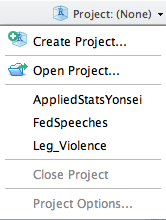
\includegraphics[width=0.3\textwidth]{/git_repositories/Rep-Res-Book/Source/Children/Chapter4/images4/ProjectMenu.png}
    \end{center}
\end{wrapfigure}


In addition to the main subdirectories of {\emph{ExampleProject}} you will probably notice a file called {\emph{README.md}} The {\emph{README.md}} file\index{README file} gives an overview of all the files in the project. It should briefly describe the project including things like its title, author(s), topic, any copyright information, and so on. It should also indicate how the folders in the project are organized and give instructions for how to reproduce the project. The README file should be in the main project folder--in our example this is called {\emph{ExampleProject}}--so that it is easy to find. If you are storing your project as a GitHub\index{GitHub} repository (see Chapter \ref{Storing}) and the file is called \texttt{README} its contents will automatically be displayed on the repository's main page. If the \texttt{README} file is written using Markdown, it will also be properly formatted. Figure \ref{BookRepository} shows an example of this.

It is good practice to dynamically include the system information for the R session you used to create the project. To do this you can write your README file with R Markdown (see Chapter \ref{LargeDocs}). Simply include the \texttt{sessionInfo()} command in a code chunk in the R Markdown document. If you knit this file immediately after knitting your presentation document it will record the information for that session.

You can also dynamically include session info in a LaTeX document. To do this use the {\tt{toLatex}} command in a code chunk. The code chunk should have the option \verb|results='asis'|. The code is:

\begin{knitrout}
\definecolor{shadecolor}{rgb}{0.969, 0.969, 0.969}\color{fgcolor}\begin{kframe}
\begin{alltt}
\hlfunctioncall{toLatex}(\hlfunctioncall{sessionInfo}())
\end{alltt}
\end{kframe}
\end{knitrout}


%% Make file discussion?

\section{Setting directories as RStudio Projects}

If you are using RStudio, you may want to organize your files as Projects\index{RStudio Projects}. You can turn a normal directory into an RStudio Project by clicking on \texttt{Project} in the RStudio menu bar and selecting \texttt{Create Project\ldots}. A new window will pop up. Select the option \texttt{Existing Directory}. Find the directory you want to turn into an RStudio Project by clicking on the \texttt{Browse} button. Finally, select \texttt{Create Project}. You will also notice in the Create Project pop up window that you can build new project directories and create a project from a directory already under version control\index{version control} (we'll do this at the end of Chapter \ref{Storing}). When you create a new project you will see that RStudio has put a file with the extension \texttt{.Rproj} into the directory.

Making your research project directories RStudio Projects is useful for a number of reasons:

\begin{itemize}
    \item the project is listed in RStudio's Project menu where it can be opened easily (see Figure \ref{ProjectMenu}).
    \item when you open the \textttt{.Rproj} file RStudio automatically sets the working directory to the project's directory and loads the workspace, history, and source code files you were last working on.
    \item you can set project specific options like whether PDF presentation documents should be compiled with Sweave or {\emph{knitr}}.
    \item when you close the project your R workspace and history are saved in the project directory,
    \item it helps you version control your files.
\end{itemize}

%%%%%%%%%%%%%%% File Manipulation
\section{R file manipulation commands}

R has a range of commands for handling and navigating through files. Including these commands in your source code files allows you to more easily replicate your actions.

\paragraph{{\tt{getwd}}}\index{getwd}

To find your current working directory use the \texttt{getwed} command:

\begin{knitrout}
\definecolor{shadecolor}{rgb}{0.969, 0.969, 0.969}\color{fgcolor}\begin{kframe}
\begin{alltt}
\hlfunctioncall{getwd}()
\end{alltt}
\begin{verbatim}
## [1] "/git_repositories/Rep-Res-Book/Source/Children/Chapter4"
\end{verbatim}
\end{kframe}
\end{knitrout}


\noindent The example here shows you the current working directory that was used while knitting this chapter.

\paragraph{{\tt{list.files}}}\index{list.files}

Use the \texttt{list.files} command to see all of the files and subdirectories in the current working directory. You can list the files in other directories too by adding the directory path as an argument to the command. 

\begin{knitrout}
\definecolor{shadecolor}{rgb}{0.969, 0.969, 0.969}\color{fgcolor}\begin{kframe}
\begin{alltt}
\hlfunctioncall{list.files}()
\end{alltt}
\begin{verbatim}
## [1] "chapter4.Rnw" "images4"
\end{verbatim}
\end{kframe}
\end{knitrout}


\noindent You can see that the \emph{Chapter4} folder has the file \emph{chapter4.Rnw} (the markup file used to create this chapter) and a child directory called \emph{images4} where I stored the original versions of the figures show in this chapter.

\paragraph{{\tt{setwd}}}\index{setwd}

The {\tt{setwd}} command sets the current working directory\index{working directory}. For example, if we are on a Mac or other Unix-like computer we can set the working directory to the {\emph{GatherSource}} directory in our Example Project (see Figure \ref{ExampleTree}) like this

\begin{knitrout}
\definecolor{shadecolor}{rgb}{0.969, 0.969, 0.969}\color{fgcolor}\begin{kframe}
\begin{alltt}
\hlfunctioncall{setwd}(\hlstring{"/ExampleProject/Data/GatherSource"})
\end{alltt}
\end{kframe}
\end{knitrout}


\noindent Now R will automatically look in the {\emph{GatherSource}} folder for files and will save new files into this folder, unless we explicitly tell it to do otherwise.

\paragraph{{\tt{dir.create}}}\index{dir.create}

Sometimes you may want to create a new directory. You can use the {\tt{dir.create}} command to do this.\footnote{Note: you will need the correct system permissions to be able to do this.} For example to create a {\emph{ExampleProject}} file in the root C directory on a Windows computer type:

\begin{knitrout}
\definecolor{shadecolor}{rgb}{0.969, 0.969, 0.969}\color{fgcolor}\begin{kframe}
\begin{alltt}
\hlfunctioncall{dir.create}(\hlstring{"C:\textbackslash{}\textbackslash{}ExampleProject"})
\end{alltt}
\end{kframe}
\end{knitrout}


\paragraph{{\tt{file.create}}}\index{file.create}

Similarly, you can create a new blank file with the \texttt{file.create} command. To add a blank R source code file called {\emph{SourceCode.R}} to the {\emph{ExampleProject}} directory on the C drive use:

\begin{knitrout}
\definecolor{shadecolor}{rgb}{0.969, 0.969, 0.969}\color{fgcolor}\begin{kframe}
\begin{alltt}
\hlfunctioncall{file.create}(\hlstring{"C:\textbackslash{}\textbackslash{}ExampleProject\textbackslash{}\textbackslash{}SourceCode.R"})
\end{alltt}
\end{kframe}
\end{knitrout}


\paragraph{{\tt{cat}}}\index{cat, R command}

If you want to create a new file and put text into it use the \texttt{cat} (concatenate and print). For example to create a new file in the current working directory called \emph{ExampleEcho.md} that includes the text ``Reproducible Research with R and RStudio'' type:

\begin{knitrout}
\definecolor{shadecolor}{rgb}{0.969, 0.969, 0.969}\color{fgcolor}\begin{kframe}
\begin{alltt}
\hlfunctioncall{cat}(\hlstring{"Reproducible Research with R and RStudio"},
    file = \hlstring{"ExampleCat.md"})
\end{alltt}
\end{kframe}
\end{knitrout}


\noindent You can use \texttt{cat} to also print the contents of a one or more objects to a file. In this example we created a Markdown formatted file by using the \texttt{.md} file extension. We could of course change the file extension to \texttt{.R} to set it as an R source code file, \texttt{.Rnw} to create a \emph{knitr} LaTeX file and so on.

The \texttt{cat} command will overwrite existing files with the new contents. To add the text to existing files use the \texttt{append = TRUE} argument.

\begin{knitrout}
\definecolor{shadecolor}{rgb}{0.969, 0.969, 0.969}\color{fgcolor}\begin{kframe}
\begin{alltt}
\hlfunctioncall{cat}(\hlstring{"More Text"}, file = \hlstring{"ExampleCat.md"},
    append = TRUE)
\end{alltt}
\end{kframe}
\end{knitrout}


\paragraph{{\tt{unlink}}}\index{unlink}

Finally, you can use the {\tt{unlink}} command to delete files and directories. 

\begin{knitrout}
\definecolor{shadecolor}{rgb}{0.969, 0.969, 0.969}\color{fgcolor}\begin{kframe}
\begin{alltt}
\hlfunctioncall{unlink}(\hlstring{"C:\textbackslash{}\textbackslash{}ExampleProject\textbackslash{}\textbackslash{}SourceCode.R"})
\end{alltt}
\end{kframe}
\end{knitrout}


\noindent \textbf{Important} the \texttt{unlink} command permanently deletes files, so be very careful using this command.

\paragraph{{\tt{file.rename}}}\index{file.rename}

You can use the \texttt{file.rename} to obviously rename a file. It can also be used to move a file from one directory to another. For example, imagine that we want to move the \emph{ExampleCat.md} file from the directory \emph{ExampleProject} to one called \emph{MarkdownFiles} that we already created.\footnote{The \texttt{file.rename} command won't create new directories. To move a file to a new directory you will need to create the directory first with \texttt{dir.create}.}

\begin{knitrout}
\definecolor{shadecolor}{rgb}{0.969, 0.969, 0.969}\color{fgcolor}\begin{kframe}
\begin{alltt}
\hlfunctioncall{file.rename}(from = \hlstring{"C:\textbackslash{}\textbackslash{}ExampleProject\textbackslash{}\textbackslash{}ExampleCat.md"}, 
            to = \hlstring{"C:\textbackslash{}\textbackslash{}MarkdownFiles\textbackslash{}\textbackslash{}ExampleCat.md"})
\end{alltt}
\end{kframe}
\end{knitrout}


\paragraph{{\tt{file.copy}}}\index{file.copy}

The \texttt{file.rename} fully moves a file from one directory to another. To copy the file to another directory use the \texttt{file.rename} command. It has the same syntax as \texttt{file.rename}:

\begin{knitrout}
\definecolor{shadecolor}{rgb}{0.969, 0.969, 0.969}\color{fgcolor}\begin{kframe}
\begin{alltt}
\hlfunctioncall{file.copy}(from = \hlstring{"C:\textbackslash{}\textbackslash{}ExampleProject\textbackslash{}\textbackslash{}ExampleCat.md"}, 
            to = \hlstring{"C:\textbackslash{}\textbackslash{}MarkdownFiles\textbackslash{}\textbackslash{}ExampleCat.md"})
\end{alltt}
\end{kframe}
\end{knitrout}


\section{Unix-like shell commands for file management} 

\begin{wrapfigure}{r}{0.5\textwidth}
    \caption{The RStudio Files Pane} %\\[0.25cm]
    \label{FilesPane}
        \begin{center}    
        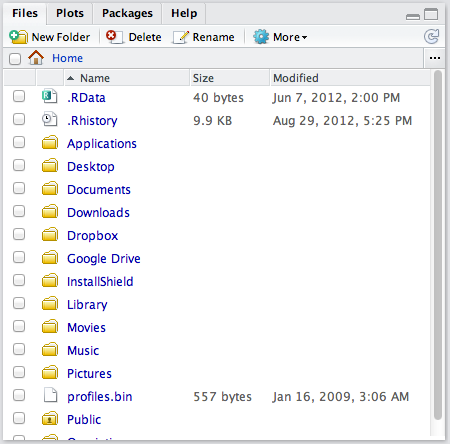
\includegraphics[width=0.45\textwidth]{/git_repositories/Rep-Res-Book/Source/Children/Chapter4/images4/RStudioFiles.png}
        \end{center}
\end{wrapfigure}

Though this book is mostly focused on using R for reproducible research it can be useful to use a Unix-like shell program\index{Unix-like shell program} to manipulate files in large projects. A command line shell program is simply a program in which you to type commands to interact with your computer's operating system. We will especially return to shell commands in the next chapter when we discuss Git\index{Git} version control and makefiles\index{makefile} for compiling large documents and batch reports\index{batch reports} as well as the command line program Pandoc (Chapter \ref{LargeDocs}). We don't have enough space to fully introduce shell programs or even all of the commands for manipulating files. We are just going to cover some of the basic and most useful commands For good introductions for Unix and Mac OS 10 computers see William E. Shotts Jr.'s book on the Linux command-line \cite[]{ShottsJr2012}. For Windows users, Microsoft maintains a tutorial on Windows PowerShell at \url{http://technet.microsoft.com/en-us/library/hh848793}. The commands discussed in this chapter should work in both Unix-like shells and Windows Powershell. That being said, I have not tested all of them in Powershell. 

It's important at this point to highlight a key difference between R and Unix-like shell syntax. In shell commands you don't need to put parentheses around your arguments. For example if I want to change my working directory to my Mac Desktop in a shell using the \texttt{cd} command I simply type:\footnote{Many shell code examples in other sources include the shell prompt, like the \texttt{\$} in Bash. It's like R's \texttt{\textgreater} prompt. I don't include the prompt in code examples in this book because you don't type them.}

\begin{knitrout}
\definecolor{shadecolor}{rgb}{0.969, 0.969, 0.969}\color{fgcolor}\begin{kframe}
\begin{verbatim}
cd /Users/Me/Desktop
\end{verbatim}
\end{kframe}
\end{knitrout}


\noindent In this example \texttt{Me} is my user name. 

\paragraph{{\tt{cd}}}\index{cd}

As we just saw, to change the working directory in the shell just use the {\tt{cd}} (change directory) command.

\paragraph{{\tt{pwd}}}\index{pwd}

To find your current working directory use the \texttt{pwd} command (present working directory). This is essentially the same as R's \texttt{getwd} command.

\begin{knitrout}
\definecolor{shadecolor}{rgb}{0.969, 0.969, 0.969}\color{fgcolor}\begin{kframe}
\begin{verbatim}
pwd

## /Users/Me/Desktop
\end{verbatim}
\end{kframe}
\end{knitrout}


\paragraph{{\tt{ls}}}\index{ls}

The \texttt{ls} (list) command works very similarly to R's \texttt{list.files} command. It shows you what is in the current working directory.

\begin{knitrout}
\definecolor{shadecolor}{rgb}{0.969, 0.969, 0.969}\color{fgcolor}\begin{kframe}
\begin{verbatim}
ls

## chapter4.Rnw images4
\end{verbatim}
\end{kframe}
\end{knitrout}


\paragraph{{\tt{mkdir}}}\index{mkdir}

Use \texttt{mkdir} to create a new directory. For example, if I wanted to create a directory in my Linux root directory called {\emph{NewDirectory}} I would type:

\begin{knitrout}
\definecolor{shadecolor}{rgb}{0.969, 0.969, 0.969}\color{fgcolor}\begin{kframe}
\begin{verbatim}
mkdir /NewDirectory
\end{verbatim}
\end{kframe}
\end{knitrout}


\noindent If running this code gives you an error message like this:

\begin{knitrout}
\definecolor{shadecolor}{rgb}{0.969, 0.969, 0.969}\color{fgcolor}\begin{kframe}
\begin{verbatim}
mkdir: /NewDirectory: Permission denied
\end{verbatim}
\end{kframe}
\end{knitrout}


\noindent you simply need to use the \texttt{sudo}\index{sudo} command to run the command with higher privileges. 

\begin{knitrout}
\definecolor{shadecolor}{rgb}{0.969, 0.969, 0.969}\color{fgcolor}\begin{kframe}
\begin{verbatim}
sudo mkdir /NewDirectory
\end{verbatim}
\end{kframe}
\end{knitrout}


\noindent Running this code will prompt you to enter your administrator password.

\paragraph{{\tt{echo}}}\index{echo}

There are a number of ways to create new files in Unix-like shells. One of the simplest ways is with the \texttt{echo} command. This command simply prints its arguments. For example:

\begin{knitrout}
\definecolor{shadecolor}{rgb}{0.969, 0.969, 0.969}\color{fgcolor}\begin{kframe}
\begin{verbatim}
echo Reproducible Research with R and RStudio
## Reproducible Research with R and RStudio
\end{verbatim}
\end{kframe}
\end{knitrout}


\noindent If you add the greater than symbol (\verb|>|) after the text you want to print then a file name, \texttt{echo} will create the file (if it doesn't already exist) in the current working directory then print the text into the file.

\begin{knitrout}
\definecolor{shadecolor}{rgb}{0.969, 0.969, 0.969}\color{fgcolor}\begin{kframe}
\begin{verbatim}
echo Reproducible Research with R and RStudio > ExampleEcho.md
\end{verbatim}
\end{kframe}
\end{knitrout}


\noindent Using only one greater than sign will completely erase the \emph{ExampleEcho.txt} file's contents and replace them with \texttt{Reproducible Research with R and RStudo}. To add the text at the end of an existing file use two greater than signs (\verb|>>|).

\begin{knitrout}
\definecolor{shadecolor}{rgb}{0.969, 0.969, 0.969}\color{fgcolor}\begin{kframe}
\begin{verbatim}
echo More text. >> ExampleEcho.md
\end{verbatim}
\end{kframe}
\end{knitrout}


\noindent There is also a \texttt{cat} shell command.\index{cat, shell command} It works slightly differently than the R version of the command and I don't cover it here.

\paragraph{{\tt{rm}}}

The {\tt{rm}}\index{rm} command is similar to R's {\tt{unlink}} command. It removes (deletes) files or directories. Again, be careful when using this command, because it permanently deletes the files or directories.

As we saw in Chapter \ref{GettingStartedRKnitr}, R also has an \texttt{rm} command. It is different because it removes objects from your R workspace rather than files from your working directory.

\begin{knitrout}
\definecolor{shadecolor}{rgb}{0.969, 0.969, 0.969}\color{fgcolor}\begin{kframe}
\begin{verbatim}
rm ExampleEcho.md
\end{verbatim}
\end{kframe}
\end{knitrout}


\paragraph{{\tt{mv}}}\index{mv}

To move a file from one directory to another with the shell use the \texttt{mv} (move) command. For example, to move the file \emph{ExampleEcho.md} from \emph{ExampleProjects} to \emph{MarkdownFiles} both in the root directory:

\begin{knitrout}
\definecolor{shadecolor}{rgb}{0.969, 0.969, 0.969}\color{fgcolor}\begin{kframe}
\begin{verbatim}
mv /ExampleProject/ExampleEcho.md /MarkdownFiles
\end{verbatim}
\end{kframe}
\end{knitrout}


\noindent Note that like the /MarkdownFiles directory must already exist. You can also use the \texttt{mv} command to simply rename files, just like the R command \texttt{file.rename}.

\paragraph{{\tt{cp}}}\index{cp}

The \texttt{mv} command completely moves a file from one directory to another. To simply copy a version of the file to a new directory use the \texttt{cp} command. The syntax is similar to \texttt{mv}:

\begin{knitrout}
\definecolor{shadecolor}{rgb}{0.969, 0.969, 0.969}\color{fgcolor}\begin{kframe}
\begin{verbatim}
cp /ExampleProject/ExampleEcho.md /MarkdownFiles
\end{verbatim}
\end{kframe}
\end{knitrout}


\paragraph{{\tt{system}} (R command)}\index{system, R command}

You can run shell commands from within R using R's \texttt{system} command. For example, to run the \texttt{echo} command from within R type:

\begin{knitrout}
\definecolor{shadecolor}{rgb}{0.969, 0.969, 0.969}\color{fgcolor}\begin{kframe}
\begin{alltt}
\hlfunctioncall{system}(\hlstring{"echo Text to Add > ExampleEcho.md"})
\end{alltt}
\end{kframe}
\end{knitrout}



\section{File navigation in RStudio}

The RStudio \textbf{Files} pane allows us to navigate and do some basic file manipulation. Figure \ref{FilesPane} shows us what this pane looks like. This pane allows us to navigate to specific files and folder, delete and rename files. To select a folder as the working directory tick the dialog box next to the file then click the \texttt{More} button and select \texttt{Set As Working Directory}. Under the \texttt{More} button you will also find options to \texttt{Move} and \texttt{Copy} files.

The \textbf{Files} pane is a GUI, so our actions in the \text{Files} pane are not as easily reproducible as the commands we learned earlier in this chapter. 

